\documentclass[11pt,jou]{apa6}
\usepackage{apacite}
\usepackage{graphicx}
\usepackage{pdfsync}
\usepackage{hyphenat}
\usepackage{verbatim}
\usepackage{multirow}
\usepackage{rotating}
\usepackage{color,soul}

% typeface command
\tolerance=500

% Prevent breaking inline formulae
\relpenalty=9999
\binoppenalty=9999



\title{Learning to compete}
\shorttitle{Learning to compete}
\author{.}
\affiliation{.}
\leftheader{.}
%\abstract{.}
%\keywords{.}

%\authornote{Brian D. Beitzel, Department of Educational Psychology,
%  Counseling and Special Education, SUNY Oneonta.
%
%  Correspondence concerning this article should be addressed to Brian
%  D. Beitzel, Department of Educational Psychology, Counseling and
%  Special Education, SUNY Oneonta, 129 Fitzelle Hall, Oneonta, NY
%  13820.  E-mail: beitzebd@oneonta.edu}

\begin{document}
\maketitle




%\section{Competition in decisions from experience}

%\cite{phillips2014rivals}

\section{Experiment 1}

\subsection{Participants and materials}

We recruited 136 participants through Amazon Mechanical Turk (www.mturk.com) using \emph{psiTurk}~\cite{gureckis2015psiturk}.
Participants were paid a base payment of \$.50 for their participation, as well as a bonus of up to \$3 depending on their performance.
Participants were randomly assigned to either the Public condition or Competitive condition (both $N=68$ or 34 pairs in each condition).

\subsection{Procedure}

\begin{figure*}[htbp]
\centerline{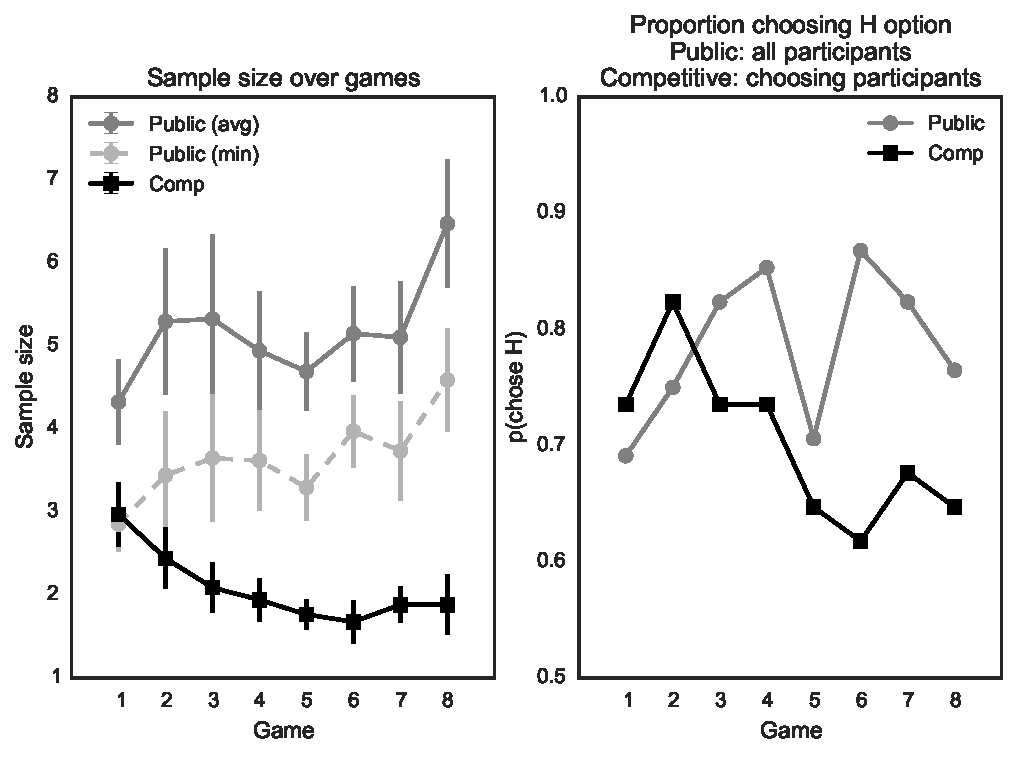
\includegraphics[width=5.5in]{figures/exp1_results.pdf}}
\caption{Experiment 1 results}
\label{exp1_results.fig}
\end{figure*}

\subsubsection{Option environment}

Each decision problem involved two options $H$ and $L$ with higher and lower expected value, respectively.
Each option was associated with two possible outcomes: a \emph{common} outcome that occurred with probability $p = .8$ and a \emph{rare} outcome that occurred with probability $1 - p = .2$.
For each option, the common outcome was a random number in the range $[-20, 20]$, while the rare outcome was a random number in the range $[-200, 200]$.
Thus, the option environment featured high-magnitude outcomes that were relatively infrequent but could have a large impact on the value of an option, including changing the sign of its perceived value (e.g., from a gain to a loss).

Twenty problem sets comprised of 8 problems each were randomly generated.
Option sets were resampled if the difference between the expected value for the $H$ and $L$ options was less than $25$. 
Problem sets were resampled if the summed expected value across all $L$ options was less than $-100$ or the summed expected value of all $H$ options was greater than $200$, ensuring that each participant's total payoff would lie in that range.

Participants were informed about the option structure, including the relative probabilities of the common and rare outcomes.
Prior to playing any games, they completed four trials of non-consequential sampling with individual options.
For each option, they were instructed to sample 25 times and observe the resulting outcome.
They then reported the highest and lowest outcomes that were seen during sampling, and estimated the expected value of the option.
All participants experienced the same four example options, which were chosen to include options where both outcomes were in the same domain (i.e., both the common and rare outcome were gains) and options where they were in different domains (i.e., a common loss but rare gain with high value).
This training ensured that participants had experience with the structure of individual options prior to the game, including the relative frequency and range of each outcome type. 
%In addition, it served as an \hl{instructional check to evaluate whether participants were able to report both outcomes they observed during sampling}.\footnote{any participants excluded based on this?}

Participants were endowed with an initial bonus of \$1.00 at the beginning of the experiment, and were instructed that their payoff from each game (the expected value of the the option they selected) would be added or subtracted when determining their final bonus.

\subsubsection{Group formation and coordination}

After completing the instructions, participants were presented with a list of open groups.
After joining an open group, they waited for a second participant to join the same group, at which point both participants confirmed that they were ready to play.
This confirmation was required for the experiment to begin to ensure that both players were present and attending to the experiment.
%At this point participants were informed that leaving experiment early would result in them forgoing any bonus payment. 

The experiment was designed such that the game advanced only when decisions were received from both players and broadcast to the entire group. 
For example, each game started when both participants confirmed they were ready to begin.
Similarly, during the sampling phase, players continued to the next trial only when they received their opponent's decision to either stop or continue sampling.

\subsubsection{Gameplay}

One of the 20 problem sets was randomly selected and played in a randomized order for each pair of participants.
On each sampling trial, a participant clicked on one of the two options (displayed as two urns filled with coins) and observed a randomly generated outcome (in the form of a coin labeled with the number of points between -200 and 200). 
The outcome remained visible until the participant indicated if they wanted to 1) ``Continue learning" or 2) ``Stop and choose." 
If both players decided to continue sampling the experiment proceeded to the next sampling trial.

If one player decided to choose an option, they then clicked on one of the two options to claim it. 
When an opponent claimed an option, an icon appeared on the other player's display indicating the choice. 
If both players decided to stop on the same trial, a random choice order was generated to determine which participant went first.

\subsubsection{Public condition}

In the public condition, a player's choices were shared with their partner but had no other consequence in terms of their ability to sample or choose.
When a player decided to stop, their selection was visible to their partner in the form of a gray person symbol that appeared below the option they chose. 
However, the partner could continue sampling for as many turns as they desired, and when they stopped could select either of the two options.
Both players were still required to acknowledge the outcome of every turn (i.e., how many players chose an option), ensuring that a player who stopped first continued to pay attention for the remainder of the game.

\subsubsection{Competitive condition}

In the competitive condition, one player's decision to stop and claim an option had the effect of removing it from the set of options available to their opponent.
When such a choice occurred, the option faded out on the display and the opponent was required to select the remaining option (thus, they were not permitted to continue sampling).
All other aspects of the gameplay were the same as in the public condition.

\subsubsection{Feedback}

There was no feedback on individual games.
At the end of the experiment, participants were shown the expected value of the options they had selected and their total bonus.


\subsection{Results}

\subsubsection{Sample size}

The observed sample size across 8 games is shown in Figure~\ref{exp1_results.fig}A.
Negative binomial regression was used to evaluate the effects of condition and game index on sample size (in the public condition, the average of the two players in each pair was used).
Sample size was higher in the public condition overall (Wald $z=-5.0$, $p<.001$).
There was a marginal positive effect of game index on sample size in the public condition ($z=1.74$, $p=.08$).
Additionally, there was a significant negative effect of game index in the competitive condition ($z=-3.4$, $p=.001$).

The decrease in sample size at the group level was evident at the level of individual pairs, with 23 pairs (68\%) in the competitive condition showing a decrease in average sample size from the first half to second half of the experiment. Of the remaining pairs, 5 (15\%) showed no change, and 6 (18\%) showed an increase in average sample size.
In comparison, participants in the public condition showed the opposite pattern of change from first to second halves of the experiment, with 21 (31\%) showing a decrease, 5 (7\%) showing no change, and 42 (62\%) showing an increase.

Notably, although the average sample size was higher in the public condition on the first game, the sample size of the first stoppers in that condition (shown by the dotted line in Figure~\ref{exp1_results.fig}A) was equivalent to the sample size observed in the competitive condition.
This suggests that participants in both conditions may have had similar strategies at the outset of the experiment, but differed in how they adjusted their information search over the course of multiple games.

%Increase in ties over games in the competitive condition, indicating convergence of strategies.



\subsubsection{Performance}

We next evaluated whether the two conditions differed in their selection of the $H$ option.
Figure~\ref{exp1_results.fig}B shows the proportion of $H$ choices for individuals in the public condition (gray line) and choosers in the competitive condition (black line).
There was a decrease in proportion of $H$ choices in the competitive condition but not the public condition.

\subsubsection{Strategy analysis}


\subsection{Discussion}

In this experiment we found that competitive pressure was associated with reduced exploration, consistent with the results of~\shortciteA{phillips2014rivals}.
Besides demonstrating the effects of competition in a different option environment, our results extend those of~\citeA{phillips2014rivals} by comparing competitive search to a ``public" condition in which participants experience the same mode of interaction (including information about other players' decisions) in the absence of competitive pressure.
Sample sizes were consistently higher in the public condition, supporting the conclusion that curtailed exploration in the competitive condition was specifically due to competitive pressure rather than some aspect of the interaction (e.g., delays due to waiting for decisions from the other player).

In addition, the results showed that the extent of information search changed over the course of repeated games.
As predicted, sample sizes decreased over games in the competitive condition, consistent with a dynamic process wherein competitors adjust how long they sample in response to competitors stopping first.
In contrast, sample sizes in the public condition had a positive trend over games, suggesting that the decrease seen in the competitive condition was not simply due to experience within the option environment.

Although ~\citeA{phillips2014rivals} did not find evidence of a reduction in sample size across games, this is likely due to the difference in option environments between experiments.
In this experiment, participants were informed as to the structure of the potential options, including the presence of a rare, potentially high-magnitude, outcome.

Interesting to note that this change in the competitive condition occurred in the absence of any feedback.


\section{Experiment 2}

\subsection{Procedure}

\subsection{Results}

\subsection{Discussion}



\section{Experiment 3}

\subsection{Procedure}

\subsection{Results}

\subsection{Discussion}


\bibliographystyle{apacite}
\bibliography{library}
\end{document}
